\documentclass{article}
\newtheorem{thm}{Theorem}
\setlength{\oddsidemargin}{0.25in}
\setlength{\textwidth}{6in}
\setlength{\topmargin}{-0.25in}
\setlength{\headheight}{0.3in}
\setlength{\headsep}{0.2in}
\setlength{\textheight}{9in}
\setlength{\footskip}{0.1in}
\usepackage{multirow}
\usepackage{fullpage}
\usepackage{graphicx}
\usepackage{amsthm}
\usepackage{amssymb}
\usepackage{url}
\usepackage{amsfonts}
\usepackage{algpseudocode}
\usepackage{mathtools}
\begin{document}	\title{ CSCI-B 565 DATA MINING \\
		Homework 2 \\
		Computer Science Core\\Spring\\Indiana University,\\ Bloomington, IN}
	\author{ Yuanzhi Bao \\ baoyu@indiana.edu}
	\date{Sept.23 2016 }
	\maketitle

\pagestyle{plain}
All the work herein is solely mine. \\ 




\subsection*{Questions}

\begin{enumerate}
\item Does $k$-means always converge? Given your answer, a bound on the iterate must be included.  How is its value determined?\\
Answer:
\begin{enumerate}
	\item $k$-means always converge but not guarantee global optimum. $k$-means need exponentially iterations if we dont give it a threshold to tell it when to stop.
	\item The bound of iterations is determined by a finit number. For the reason that $k$-means will difinetly give us a converger result. We can set up a large number based on the dataset we are facing so when the iteration number hits the number, $k$-means can stop.
\end{enumerate}
\item \textsc{Lines} 12-16 of the $k$-means algorithm describe initialization of the centroids.  Why is this code problematic?  What are some implications of using $k$-means?   \\
Answer:\\
\begin{enumerate}
	\item We don't know $k$-value at first, all we can do is guessing, which makes this code problmatic.
	\item
	\begin{enumerate}
		\item Advantages
		\begin{enumerate}
			\item If we have a large set of base number, then $k$-means would easily give us a faster computational result then hierarchical clustering.
			\item $k$-means could give us a tighter clusters then hierarchical clustering, especially when the clusters are globular.
		\end{enumerate}
		\item Disadventages
		\begin{enumerate}
			\item It's very difficult to predict k value
			\item It doesn't work well with global cluster.
			\item It could end up with different results when we gave different initial partitions.
			\item It's a NP hard cluster, which means even if we get a good result, we still dont know if there is better result out there.
		\end{enumerate}
	\end{enumerate}
\end{enumerate}
\item What is the run-time of this algorithm (include your new parameter from Question 1).\\
Answer:\\
$O(n * K * I)$\\
n: number of points\\
k: number of clusters\\
I: number of iterations\\
\item We describe two problems that arise when using $k$-means in practice.  Assume the datum is $\delta\in\Delta$, the centroids are $c_i, c_j$ for $i\neq j$ and distance $d$.  
\begin{itemize}
\item {\it Ties} occur when $d(c_i, \delta) = d(c_j, \delta)$.  Of course, there can be threeway, fourway, $\ldots$, $k$-way ties.  One solution is to randomly assign the datum to one of the two centroids.   What are two other solutions to this problem?\\
Answer:
\begin{enumerate}
	\item We can simply assign the datum to the "first best", which means when $Ties$ happens, just assin the datum to the first one.
	\item We can also simply assign the datum to the "last best", which means when $Ties$ happens, just assin the datum to the last one.
\end{enumerate}
\item {\it Centroid collapse} occurs when $d(c_i, c_j) \sim 0$. Like ties, this can include more than two.  One is to find the median $m$ of the union of the two centroids and then assign values less than the median to one and values greater than the median to the other, taking into account an odd number will be the problem above.  What are two other solutions?  Observe that an additional threshold on centroids, $\tau_c > 0$, is needed, to determine whether $d(c_i, c_j) \leq \tau_c$ is true.  First, how would $\tau_c$ be determined?  Second, where in the algorithm should this be checked?\\
Answer:\\
\begin{enumerate}
	\item Two other solutions:
	\begin{enumerate}
		\item We can simply just delete all the other same centroids and assign the all data to just one.
		\item We can also just ramdonly pick $1/n$ (n is the number of the same centroids) to every centroids which have tha same value
	\end{enumerate}
	\item To detemrmine $\tau_c$ is as same as to determine how seperate you want to centtroids to be.\\
	If you want them to be more seperate than $\tau_c$  should be reasonly big, otherwise $\tau_c$  should be reasonly small.\\
	\item It should be  before we update centriods with average. So we can implement this before line 25 and after line 24
\end{enumerate}
\item Modify the $k$-means algorithm to address ties and collapsing centroids.  Explicitly add pseudo-code to the algorithm and call this $k$-meansr. 
{\small
	\begin{center}
		\begin{algorithmic}[1]\label{kmeansr}
			\State{\bf ALGORITHM} \texttt{k-meansr}
			\State {\bf INPUT} (\textsf{data} $\Delta$, distance $d:\Delta^2\rightarrow \mathbb{R}_{\geq 0}$, \textsf{centoid number} $k$, \textsf{threshold} $\tau$)
			\State {\bf OUTPUT} (\textsf{Set of centoids} $\{c_1, c_2, \ldots, c_k\}$)
			\State
			\State \texttt{***} $Dom(\Delta)$ denotes domain of data.
			\State
			\State \texttt{***} Assume centroid is structure $c = (v \in DOM(\Delta), B\subseteq \Delta)$
			\State  \texttt{***} $c.v$ is the centroid value and $c.B$ is the set of nearest points.
			\State \texttt{***}  $c^{i}$ means centroid at $i^{th}$ iteration. 
			\State
			\State $i = 0$
			\State \texttt{***} Initialize Centroids
			\For{$j = 1,k$}
			\State $c_j^i.v \gets  random(Dom(\Delta))$
			\State $c_j^i.B \gets \emptyset$
			\EndFor
			\State
			\Repeat
			\State $i \gets i + 1$
			\State \texttt{***} Assign data point to {\it nearest} centroid
			\For {$\delta \in \Delta$}
			\If there are more than one min centroids which $d(\delta, c_j^i.v) = d(\delta, c_k^i.v)$
			\State $r \gets$ random chose one from all the centroids which have the same $d$
			\State $c_r^i.B \gets c.B \cup \{\delta\}$
			\Else
			\State $c_j^i.B \gets c.B \cup \{\delta\}$, where $\min_{c_j^i}\{d(\delta, c_j^i.v)\}$
			\EndIf
			\EndFor
			\For {$j = 1, k$}
			\State \texttt{***} Check for $Centroid \ collaspe$
			\If  There are more than one centroids $d(c_i, c_j) \sim 0$
			\State Randomly choose $1/n$(n is the number of the centriods) to every centriods.
			\EndIf
			\State \texttt{***} Get size of centroid
			\State $n \gets |c_j^i.B|$
			\State \texttt{***} Update centroid with average 
			\State $c_j^i.v \gets (1/n)\sum_{\delta \in c_j^i.B} \delta$
			\State \texttt{***} Remove data from centroid
			\State $c_j^i.B \gets \emptyset$
			\EndFor
			\State \texttt{***} Calculate scalar product (abuse notation and structure slightly)
			\State \texttt{***} See notes
			\Until{$((1/k)\sum_{j=1}^k~|| c^{i-1}_j-c^{i}_j||) < \tau$}
			\State {\bf return} ($\{c_1^i, c_2^i, \ldots, c_k^i\}$) 
			\end{algorithmic}
	\end{center}}
\end{itemize}
\end{enumerate}

\subsection*{Integration}
We will look at the problem of integrating two pieces of data through a metric.  The data are described by $([X:t], d_x), ([Y:u], d_u)$ where $X:t$ means it is type $t$,  $Y:u$ is type $u$, and $d_x,d_y$ distance metrics.  We integrate the data and now need a metric $([X:t]\times [Y:u], d)$.  Is this possible?  We need to prove  that $d$ is a metric.  To make notation easier, assume $Z = [X:t]\times [Y:u]$.  For $(a,b) \in Z^2$, we write $a_0$ to mean the $t$ type leftside of the product and $b_0$ for the $t$ type rightside.  For example, $Z = [N : \textsf{int}] \times [S : \textsf{string}]$.  $(a,b) = ((34, \texttt{two}), (100, \texttt{three}))$, then $a_0 = 34, b_0 = 100$ and $a_1 = \texttt{two}, b_1 = \texttt{three}$.

Let's define one of the simplest metrics.
$d:Z^2 \rightarrow \mathbb{R}_{\geq 0}$ where:
\begin{eqnarray*}
d(a,b) &=& d_x(a_0,b_0) + d_y(a_1,b_1)
\end{eqnarray*}
Now we show reflexivity, symmetry, and transitivity.  
\begin{itemize}
\item $(\forall, a \in Z)\ d(a,a) = 0$.  Then $d(a,a) = d_x(a_0,a_0) + d_y(a_1,a_1) = 0$  
\item $(\forall\, a, b)\ d(a,b) \rightarrow d(b,a)$.    
\[ d(a,b) = d_x(a_0,b_0) + d_y(a_1,b_1) = d_x(b_0,a_0) + d_x(b_1,a_1) = d(b,a) \]
\item $(\forall\, a,b,c)\ d(a,b) + d(b,c) \geq d(a,c)$
\begin{eqnarray*}
d(a,b) + d(b,c) &=& d_x(a_0,b_0) + d_x(b_0,c_0) + d_y(a_1,b_1) + d_y(b_1,c_1)\\
&\geq& d_x(a_0,c_0) + d_y(a_1,c_1) = d(a,c)\\
\end{eqnarray*}
\end{itemize} 

Suppose we have $[X:\textsf{int}]$ are the number of cable subscription cancelations (say, {\it per} hour).  We find data $[Y:\textsf{char}]$ that  indicates whether there was  ``good'' programming at that time (we're purposely being vague).  The ordering is $\texttt{n} < \texttt{o} <  \texttt{g} < \texttt{e}$, $\texttt{e}$ being the best.  We integrate this and get:
\begin{center}
\begin{tabular}{cc}
$X$ & $Y$ \\ \hline \hline
14 & \texttt{g} \\
 45 & \texttt{o} \\
 54 & \texttt{g} \\
 21 & \texttt{n} \\
 60 & \texttt{o}
 \end{tabular}
 \end{center}
 Although we didn't need to use the type information explicitly, its presence shows that we can build metrics over disparate kinds of integrated data.   Design a simple metric, different from the one above, for this integrated data.  Prove it is a metric.\\
 Answer:\\
 \begin{enumerate}
 	\item Design a simple metric:
 	\begin{enumerate}
 		\item We can assume that\\ 
 		\begin{eqnarray}
 	d_x(i,j) &=& \left\{\begin{array}{l} 0,\ \ \ i = j \\ 1,\ \ \  i\neq j \end{array}\right.\ \ \ \mbox{For objects $i,j$}. \\
 		\end{eqnarray}
	 		\begin{eqnarray}
 			d_y(i,j) &=& \left\{\begin{array}{l} 0,\ \ \ i = j \\ 1,\ \ \  i\neq j \end{array}\right.\ \ \ \mbox{For objects $i,j$}. \\
 			\end{eqnarray}
 		\item The integrate matric
 		\begin{eqnarray*}
 			d(a,b) &=& d_x(a_0,b_0) + 3 * d_y(a_1,b_1)
 		\end{eqnarray*}
 		
 	\end{enumerate}
 	\item Prove:
 	\begin{enumerate}
 		\item refexivity: This is obvious\\
 		$(\forall, a \in Z)\ d(a,a) = 0$.  Then $d(a,a) = d_x(a_0,a_0) + 3 * d_y(a_1,a_1) = 0$  
 		\item symmetry: This is obvious too\\
 		$(\forall\, a, b)\ d(a,b) \rightarrow d(b,a)$.    
 		\[ d(a,b) = d_x(a_0,b_0) + 3 * d_y(a_1,b_1) = d_x(b_0,a_0) + 3 * d_y(b_1,a_1) = d(b,a) \]
 		\item transitivity:\\
 		$(\forall\, a,b,c)\ d(a,b) + d(b,c) \geq d(a,c)$\\
	 	$d(a,b) = d_x(a_i,b_i) + 3 * d_y(a_j,b_j) $\\
	 	$d(b,c) = d_x(b_i,c_i) + 3 * d_y(b_j,c_j) $\\
	 	$d(a,c) = d_x(a_i,c_i) + 3 * d_y(a_j,c_j) $\\
	 	Based on the matric above we can simplify the provef to prove\\ $d(a,b) + d(b,c) \geq d(a,c)$\\
	 	if $a = b = c$\\
	 	$d(a,b) + d(b,c) = d(a,c) =  0$\\
	 	if $a \neq b \neq c$\\
	 	$d(a,b) + d(b,c ) = 2 > d(a,c)$ \\
	 	if $a \neq b, b\neq c, a\neq c$\\
	 	$d(a,b) + d(b,c) = 2 > d(a,c)= 0$\\
		There is impossbile that $a = b, b = c, a \neq c$ 
		So it has transitivity.
 	\end{enumerate}
 \end{enumerate}
\begin{enumerate}
\item  We can combine multiple metrics to built more sophisticated measures of dissimilarity. This problem has to do with different metrics over the same data.  Let  $x = \{a,b,c,d\}, y = \{a, b, e\}, z = \{b, f\}, w = \{a,d,f,e\}$.  Here are several metrics:

 \begin{eqnarray*}
 d_1(x,y) &=& \left\{\begin{array}{l} 0,\ \ \ x = y \\ 1,\ \ \  x\neq y \end{array}\right.\ \ \ \mbox{For objects $x,y$}. \\
 &&\\
 J(x,y) &=&|x \cap y|/|x \cup y|\ \ \ \mbox{\rm For sets $x,y$.} \\   d_2(x,y) &=& 1-J(x,y)\ \ \ \mbox{\rm For sets $x,y$.}\\
 &&\\
c(x,y) &=& \left\{\begin{array}{l}0, \ \ \ x = y\\ 1, \ \ \ otherwise\end{array}\right. \mbox{\rm for individual characters, {\it e.g.}, \texttt{a} = \texttt{b}}\\
d_3(\mathrm{\bf x},\mathrm{\bf y}) &=& \Sigma_{i=0}^{n-1}c(\mathrm{\bf x}[i], \mathrm{\bf y}[i]) \ \ \ \ n = ||\mathrm{\bf x}||, \mbox{\rm the length of the string.}\\
&&\\
d_4(\mathbf{x},\mathbf{y}) &=& \left|{\frac{\mathbf{x}^{\mathsf{T}}\mathbf{y}}{||\mathbf{x}||\,||\mathbf{y}||}}\right| \ \ \ \mbox{\rm for vectors $\mathbf{x}, \mathbf{y} \in \mathbb{R}^n$} 
 \end{eqnarray*}
 
Calculate the following:
\begin{enumerate} \item For every $i$, find $d_i(x,w)$\\
	$d_1(x, w) = 0 $ Since the x, w don't contain the same elements\\
	$d_2(x, w) = 1- 1/ 3 = 2/3$\\
	$d_3(x, w) = 0 + 1 + 1 + 1 = 3$\\
	$d_4(x, w) = (a^2 + bd + cf + ed) / (\sqrt{a^2 + b^2 + c^2 + d^2} * \sqrt{a^2 + d^2 + f^2 + e^2})$
	 \item Find the $d_i$ that has the minimum value for $x,z$.\\
	 \begin{enumerate}
	 	\item $d_1(x,z) = 1$
	 	\item $d_2(x,z) = 1 - 1/5 = 4 /5$
	 	\item $d_3(x,z) > 1$
	 	\item $d_4(x,z)$ is a range of 0 to 1
	 	\item Conclusion:\\
	 	Since $d_2$ is for sure number $d_4$ is not. The minimum value shoule be $d_2$
	 \end{enumerate}
	   \item Which distance gives the the maximum value for any pairs? \\
	   Answer:\\
	   $d_3$ gives the maximum value for any pairs for the reason that others all have the limitation of 1, but $d_3$ gives value bigger than 1
	    \item \textsf{True or False}.  For any set $v$, $d_1(v,v) = d_2(v,v) = d_3(v,v) = d_4(v,v)$.\\
	    Answer:\\
	    False\\
	    look at the \(a\) problem we can say it's false.
	     \end{enumerate}

\item We have shown that metrics can be combined.  Why is the important to integration? Prove or disprove the following are metrics (using $d_i$ from above):\\
Answer:\\
For the reason that when we intergration different sets, we can have the distance between different sets. For this reason we can combine different features that represent one data. So we can make more accurate answer or sophisticated answer.\\
To prove or disprove the following are matrics we have to prove $d_1\ to\ d_4$ is matric or not. The prove statement are show following.
\begin{enumerate}
	\item $d_1$
	\begin{enumerate}
		\item refexivity:\\
		$d_1(a,a) = 0$\\
		\item symmetry: :\\
		if $a = b$\\
		$d_1(a, b) = d_1(b, a) = 0$\\
		if $a \neq b$\\
		$d_1(a,b) = d_1(b,a ) = 1$\\
		proved\\
		\item transitivity:\\
		if $a = b = c$ \\
		$d_1(a,c) = d_1(a,b) + d_1(b, c) = 0$\\
		if $a \neq b \neq c$\\
		$d_1(a,c) = 1 < d_1(a,b) + d_1(b, c) = 2$\\
		if $a \neq b = c$ or $a = b \neq c$ \\
		$d_1(a,c) = 1 = d_1(a,b) + d_1(b, c) = 1$\\
		proved
	\end{enumerate}
	\item $d_2$
	\begin{enumerate}
		\item refexivity:\\
		$d_2(a,a) = 0$\\
		\item symmetry: :\\
		$d_2(a,b) = d_2(b,a)$ for the reason the same elements in two sets won't change when they change the order. So the answer remind the same.\\
		\item transitivity:\\
		As we know its Jaccard distance, we can say that\\
		$d_2(a,b) + d_2(b,c) \geq d_2(a,c)$\\
	\end{enumerate}
	\item $d_3$
		\begin{enumerate}
			\item For the reason that if $x$ and $y$ are not the same length, $d_3$ became a not well defined "metric". Which made it not a metric.
		\end{enumerate}
		\item $d_4$
		\begin{enumerate}
			\item refexivity:\\
			$d(a,a) = 1$\\
			So it's not a metric.
		\end{enumerate}
\end{enumerate}
Now we can prove or disprove follows are metric or not
\begin{enumerate}
\item $d_{i'}(x,y) = \frac{d_i(x,y)}{1 + d_i(x,y)}$ for every $i$.\\
\begin{enumerate}
	\item $d_1$
	\begin{enumerate}
		\item refexivity:\\
		$d(a,a) = \frac{d_(a,a)}{1 + d_(a,a)} = \frac{0}{1+0} = 0$\\
		proved
		\item symmetry: \\
		if $a = b$\\
		$d(a,b) = d(b,a) = 0$
		if $a\neq b$\\
		$d(a,b) = d(b,a) = 1/2$\\
		proved
		\item transitivity:\\
		if $a = b = c$\\
		$d(a,b) = d(b,a) = d(a,c) = 0$\\
		if $a \neq b = c$\\
		$d(a,b)  + d(b, c) = 1/2 + 0 = 1/2 > d(a,c) = 0$\\
		if $a \neq b \neq c$\\
		$d(a,b)  + d(b, c) = 1/2 + 1/2 = 1 > d(a,c) = 1/2$\\
		if $a = b \neq c$\\
		$d(a,b)  + d(b, c) = 0 + 1/2 = 1/2 = d(a,c) = 1/2$\\
		proved
		So all cases $a,b,c$\\
		We have $d_1$ is a metric \\
	\end{enumerate}
	\item $d_2$\\
	\begin{enumerate}
		\item refexivity:\\
		$d(a,a) = \frac{d_(a,a)}{1 + d_(a,a)} = \frac{0}{1+0} = 0$\\
		proved
		\item symmetry: \\
		if $a = b$\\
		$d(a,b) = d(b,a) = 0$
		if $a\neq b$\\
		$d(a,b) = d(b,a) \neq 0$\\
		proved
		\item transitivity:\\
		The only way I can demenstrate is based on it is metric as $d_2$, $d_{i'}(a,b)$ keeps the basic as $d_2$. So we can say it is refexivity proved.\\
	\end{enumerate}
	\item $d_3$\\
		It's not a metric because it is not well defined, as x, y have different length we don't know what to do.
	\item $d_4$\\
		It's not a metric because $d(a,a) \neq 0$
\end{enumerate}
\item $d_{i'}(x,y) = \alpha d_i(x,y)$ for $\alpha\in\mathbb{R}_{>0}$\\
\begin{enumerate}
	\item $d_1$
	\begin{enumerate}
		\item refexivity:\\
		$\alpha d(a,a) = \alpha * 0 $\\
		proved
		\item symmetry: \\
		if $a = b$\\
		$\alpha * d(a,b) = \alpha * d(b,a) = 0$\\
		if $a\neq b$\\
		$\alpha * d(a,b) = \alpha * d(b,a) \neq 0$, we know they are equal but value is variety based on different data sets.\\
		proved
		\item transitivity:\\
		if $a = b = c$\\
		$\alpha * d(a,b) =\alpha d(b,a) = \alpha d(a,c) = 0$\\
		if $a \neq b = c$\\
		$\alpha * d(a,b)  + \alpha*d(b, c) = \alpha * 1 + 0 = \alpha > d(a,c) = 0$\\
		if $a \neq b \neq c$\\
		$\alpha * d(a,b)  + \alpha*d(b, c) = \alpha * 1 + \alpha * 1 = \alpha * 2 >  d(a,c) = \alpha$ Since $\alpha > 0$\\
		if $a = b \neq c$\\
		$\alpha * d(a,b)  + \alpha*d(b, c) = 0 + \alpha * 1 = \alpha  =  d(a,c) = \alpha$ \\
		proved
		So all cases $a,b,c$\\
		We have $d_1$ is a metric \\
	\end{enumerate}
	\item $d_2$\\
	\begin{enumerate}
		\item refexivity:\\
		Since $d_2$ satisfies this qulity, multiple with$ \alpha > 0 $ will keep this qulity.
		proved
		\item symmetry: \\
		if $a = b$\\
		$\alpha * d(a,b) = \alpha * d(b,a) = 0$
		if $a\neq b$\\
		$d(a,b) = d(b,a) \neq 0$\\
		proved
		\item transivity:\\
		The only way I can demenstrate is based on it is metric as $d_2$, $d_{i'}(a,b)$ keeps the basic as $d_2$. So we can say it is refexivity proved.\\
	\end{enumerate}
	\item $d_3$\\
	It's not a metric because it is not well defined, as x, y have different length we don't know what to do.
	\item $d_4$\\
	It's not a metric because $\alpha * d(a,a) \neq 0$
\end{enumerate}
\item $d_5(x,y) = d_1(x,y) + 3d_2(x,y)$\\
It is metric
\begin{enumerate}
	\item refexivity:\\
	$d_1(a, a) + 3d_2(a,a) = 0 + 0 = 0$\\
	proved
	\item symmetry: \\
	if $a = b$\\
	$d_1(a,b) + 3 *d_2(a,b) = 0 + 0 = 0$\\
	if $a\neq b$\\
	$d_1(a,b) + 3 *d_2(a,b) = 1 + 3 * m$ we dont know this m, but $d_2(a,b) = d_2(b,c)$ based on aboved
	$d_1(a,b) + 3 *d_2(a,b) = 1 + 3 * m$
	proved
	\item transitivity:\\
	Based on we already know that $\alpha*d_2(a,b)$ is valide, $d_1(a,b) + 3 * d_3(a, b)$ doesn't change the quality of this two metrics, we can say it still transitivity.
\end{enumerate}
\item $d_6(x,y) = d_2(y,x)$\\
It is metric since change the positions of x, y wont change the property of $d_2$
\item $d_7(x,y) = d_3(x,y)d_2(x,y)$\\
It is not metric since $d_3$ is not well difined as we mentioned above
\item $d_8(x,y) = \sum_{i=1}^{4}d(x,y)$\\
it is Not metric since $d_3$ and $d_4$ are not metric, sum up them wont change their property. Specially $d_3$ is not well defined.
\end{enumerate}
\item Read the paper, ``A Survey on Tree Edit Distance and Related Problems,'' by Bille\cite{Bille:2005:STE:1085274.1085283}.  In no more than two paragraphs, discuss what is {\it most} relevant to either datamining or data science.\\
Answer:\\
In either datamining or data science we have the following relevant important directions based on the paper:\\
The problems we are talking about here are tree edit distance, alignment distance, and inclusion problems. So when we talk about problems we are talking about these.\\
\begin{enumerate}
	\item There are some orderred versinos of the problems above are NP-complete. Using defferent types of mappings would give these NP-complete problem a lot improvement of understandng.
	\item We now have the lower bound and woesr upper bound for the ordered tree edit distance, But there is a big gap between these two which means we have a lot work to do to improve this.
	\item We should consider more than edit operations other than the operations mentioned above. 
\end{enumerate}
\end{enumerate}







\section*{Application of $k$-means and Data Prepartion to Medical Data}

 This problem examines Wolberg's breast cancer data\cite{WMbreast90} that we will denote by $\Delta$. This set, though tiny, provides a good start for $k$-means and preprocessing. $\Delta$ is found at\\
  {\texttt {http://archive.ics.uci.edu/ml/machine-learning-databases/breast-cancer-wisconsin/}}\\
  
  \begin{tabular}[h]{l||l}
data & {\texttt{breast-cancer-wisconsin.data}}\\ \hline 
description &  {\texttt{breast-cancer-wisconsin.names}}  
\end{tabular}

While you will read the data description to more fully understand the format, we create some attribute names to make discussion easier.


\begin{center}
\begin{tabular}[h]{rrrr}
\textsf{ID} & \textsf{Description} & \textsf{Domain} & \textsf{Attribute Name} \\ \hline \hline
 1. & Sample code number        &    string & SCN \\ 
   2.& Clump Thickness             &  $\mathbb{N}$ & $A_2$ \\
   3.& Uniformity of Cell Size     &  $\mathbb{N}$ & $A_3$\\
   4.& Uniformity of Cell Shape  &   $\mathbb{N}$ & $A_4$\\
   5.& Marginal Adhesion           &  $\mathbb{N}$ & $A_5$\\
   6.& Single Epithelial Cell Size  & $\mathbb{N}$ & $A_6$\\
   7.& Bare Nuclei                  & $\mathbb{N}$ & $A_7$\\
   8.& Bland Chromatin          &     $\mathbb{N}$ & $A_8$\\
   9.& Normal Nucleoli           &    $\mathbb{N}$ & $A_9$\\
  10.& Mitoses                       & $\mathbb{N}$ & $A_{10}$\\
  11.& Class:                       & char &  $C$ \\ \hline 
  \end{tabular}
\end{center}

\begin{enumerate}\item  {\bf Datamining Problem} Suppose you're working to help a clinic serve a community that has limited resources to identify and treat breast cancer.  The cost of a biopsy is from \$1000 to \$5000, since it requires a pathologist.  The cost of a masectomy is \$15,000 to \$55,000 (these are representative costs in 2016).   The cost of a computer program, ignoring the modest fixed cost of machine {\it etc.}, is \$10.

 \begin{enumerate} \item What is the total cost of the biopsies in $\Delta$ when done by a pathologist?  Assume the computer can identify 90\% of the cases to nearly 100\% accuracy.  What is the cost of the computer program? \\
 	Answer:\\
 	The reason I can only give a range for this question is because we dont know what excatly cost for every one. So a range is a reasonable answer. I know someone may use mean as the number. But for human elements we should be careful about this.
 	\begin{enumerate}
 		\item We have 669 instances in this data set so the cost is between $1000 * 669$ to $5000 * 669$ is $669000\$$ to $3345000\$$  
 		\item As we know now cumpyter give $90\%$ right answer. Which means everytime computer runs the program, only $10\%$ is wrong. For a single point it has $10\%$ get the wrong answer. So if we run the program three times. For each single  point which doesn't change the reasult for this three times. It would be only $10\% * 10\% * 10\%$ is $0.1\%$ to get the wrong answer. Which give us the confidence to say it's right.\\
 		So the cost for this strategy is $10\$ * 669 * 3 = 20070\$$
 	\end{enumerate}
 	\item What would have been the likely total cost of masectomies?\\
 	Answer:\\
 	Cost = $15000 * number\ of\ Malignant $ to $55000 * number\ of\ Malignant $ = $3615000$ to $13255000$
 	 \item Assuming a 70\% mortality rate for untreated in year five, how many deaths does the data suggest in five years? \\
 	 Answer:\\
 	 We have the $10\%$ wrong number is we dont exam the data serveral times.\\
 	 result = $10\% * number\ of\ Benign * 70\% = 0.1*458*0.7 =  32$
 	 \item Compose a succint problem statement that you imagine is pertinent to this scenario. \\
 	 Answer:\\
 	 From my perspect, the result of computer can not be trusted 100\%. So the best way to solve this problem is to combine computer and human pathologist. Let the computer learn to decide the result it can be positive sure but pass the unsure data to the human pathologist.\\
 	 Also It is not just bi or ma. Some people condition is between these two.
 	 \end{enumerate} \item {\bf Data Preparation} Ignoring the \texttt{Sample code number} (SCN), \begin{enumerate} \item Ignoring the SCN and $C$ columns, how many attributes (or features) does $\Delta$ have? \\
 	 Answer:\\
 	 9 features
 	 \item Let $\Delta^{miss}\subset \Delta$ be the data that has missing values.  How many missing values exist (total)?  What is the size of $\Delta^{miss}$? \\
 	 Answer:\\
 	 \begin{enumerate}
 	 	\item only one missing value exist. it's the valule of Bare Nuclei
 	 	\item 16 points have the missing value. \\
 	 	$\Delta^{miss} = 16$
 	 \end{enumerate}
 	 \item How many patients have missing values?\\
 	 Answer:\\
 	 16
 	  \item Give the SCNs for that have missing values.  \\
 	  1057013 1096800 1183246 1184840 1193683 1197510 1241232  169356  432809  563649  606140   61634  704168  733639 1238464 1057067
 	  \item Of these data, would you have recommended re-examination for the women?  What would be the costs both for the pathologist and computer program? \\
 	  \begin{enumerate}
 	  	\item  I would like to recommended re-exnimation these data. For the reason that based on later data Correlation Coefficient  Uniformity of Cell Shape is the one shoule be deleted, which means this data is relavantly important.\\
 	  	\item 
 	  	The cost for pathologist:\\
 	  	$1000 * 16$ to $5000 * 16$ is $16000\$$ to $80000\$$\\
 	  	The cost for computer:\\
 	  	$10 * 16 = 160$\\ 
 	  \end{enumerate}
 	  
  \item Is the amount of missing data significant from an algorithmic perspective? \\
  Answer:\\
  Based on the statement above I would say it's not significant from an algorithmic perspective. For the reason that the result not defined just by one value, but by all the 9 values. Missing one of them won't change the result significanly based on what I tried later in the K-means algorithm.
  \item Assess the significance of either keeping or removing the tuples with unknown data. You should consider the human element too.\\
  Answer:\\
  \begin{enumerate}
  	\item At first it seems like it's not siginificance if we just remove the tuples with unknow data. For the reason that in almost 700 data lose 16 is not matter. 
  	\item In this assignment, I did remove the tuples with unknow data in the K-means implement at first and got a very good result. 95\% correct. The reason I did this is just because it would gave us a better and more clear answer if we just removed the "imperfect" data.
  	\item But we should consider this in different situations. For example 16 may seem like a small number when it compare to 700 but if these 16 people have different situation than others, Then they become significant for the whole data.
  	\item In the mean while, They are real people. We should not just removing they like that. At least we could fix the data or found out the reason they have unknow data.
  \end{enumerate}
 \item Repair $\Delta^{miss}$ by replacing unknown data using one of the techniques we discussed in class.  This will be  presented as $(\texttt{SCN}, A_i, v)$ where \texttt{SCN} is the tuple key, $A_i$ is the attribute, and $v$ is the new value.
 Create a \texttt{CSV} file \texttt{DeltaFix.csv} for this data.  Call the entire data set, including the values that have been replaced, as $\Delta_1^{clean}$.\\
 Answer:\\
 Using the mean of  the feater in the all data that with no-missing value to implement the missing value. The fixed data is as below:
 \begin{center}
 	\begin{tabular}{ccc}
 		$SCN$ & $A_i$ & $v$\\ \hline \hline
 		 1057013 & $A_7$ & 4\\
 		  1096800  & $A_7$ & 4\\
 		 1183246  & $A_7$ & 4\\
 		 1184840  & $A_7$ & 4\\
 		1193683  & $A_7$ & 4\\
 		 1197510  & $A_7$ & 4\\
 		1241232  & $A_7$ & 4\\
 		   169356 & $A_7$ & 4\\
 		  432809  & $A_7$ & 4\\
 		  563649  & $A_7$ & 4\\
 		  606140 & $A_7$ & 4\\
 		   61634  & $A_7$ & 4\\
 		  704168  & $A_7$ & 4\\
         733639  & $A_7$ & 4\\
 		 1238464  & $A_7$ & 4\\
 		 1057067  & $A_7$ & 4\\
 	\end{tabular}
 \end{center}
 \end{enumerate} 
 
  \item {\bf Data Analysis}
   \begin{enumerate} \item Using either \texttt{MySQL}, \texttt{SQL Server} or \texttt{PostgreSQL}, built a table and load the fixed data set.  Connect to \texttt{R} so that you can quickly and easily perform analysis.  Using \texttt{R}, 
\item Plot histograms for each attribute and $C$.\\
\begin{figure}[h]
\centering
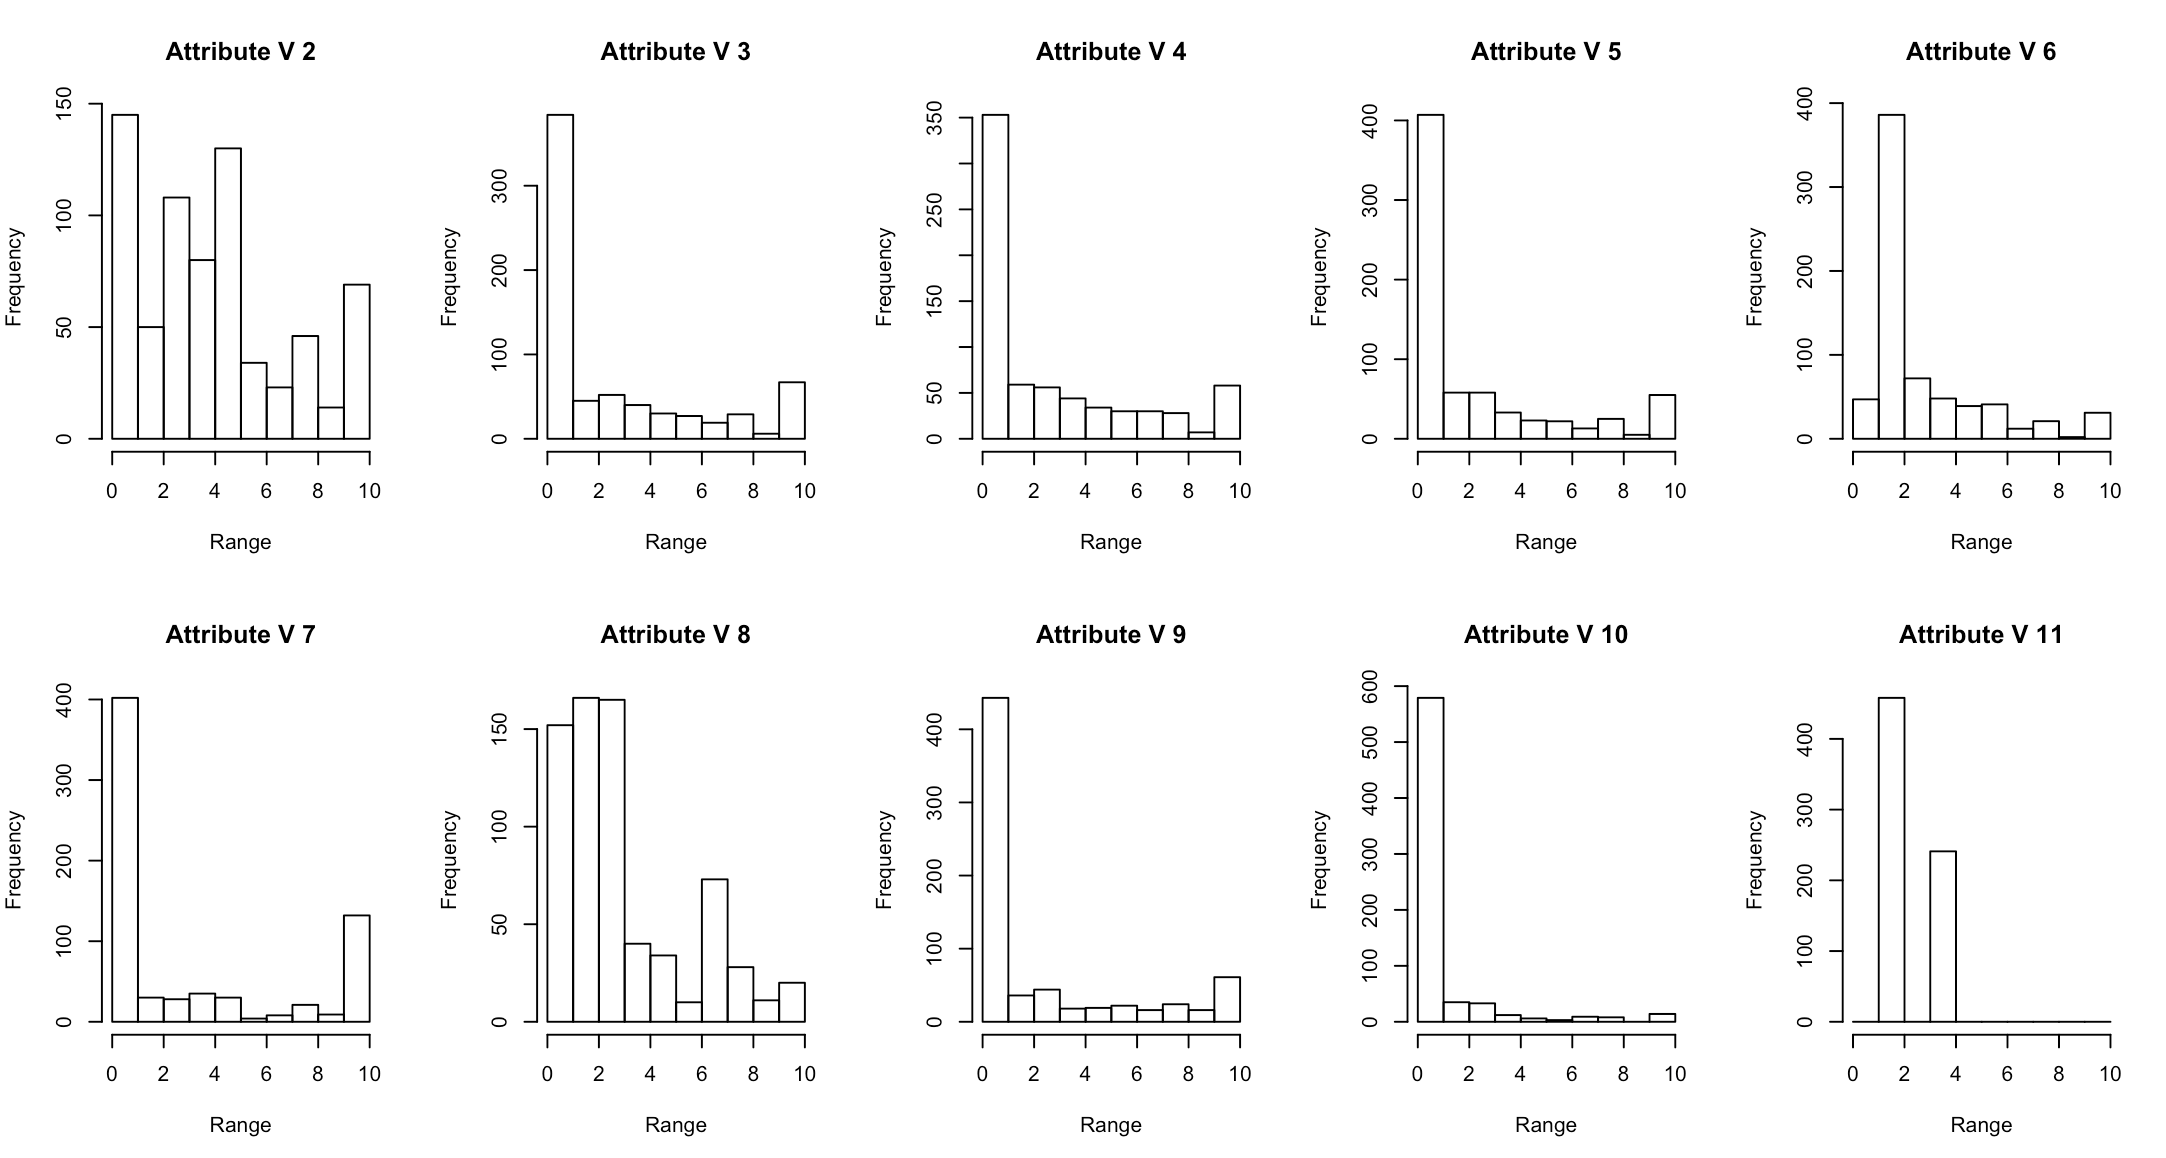
\includegraphics[width=0.7\linewidth]{histforallvalue}
\caption{}
\label{fig:histforallvalue}
\end{figure}

 \item Find the mean, median, mode, and variance of each attribute.\\
 Answer:\\
 The code are writen in R file saved in matrix C
  \begin{center}
  	\begin{tabular}{ccccc}
     $A_i$ & mean&median&mode&variance\\ \hline \hline         
    $A_i$&4.417 &4 &1 &7.92\\
     $A_i$&3.13&1 &1&9.31\\
    $A_i$ &3.20&1&1 &8.83\\
    $A_i$ &2.80 &1 &1 &8.15\\
     $A_i$ &3.21&2 &2&4.90\\
    $A_i$ &3.55&1&1&12.97\\
    $A_i$ &3.43&3&2&5.94\\
    $A_i$ &2.86 &1&1&9.32\\
    $A_i$ &1.58 &1&1&2.94\\
    	\end{tabular}
    \end{center}
 \item For each pair $A_i, A_j$, $i \neq j$, find the Pearson's correlation coefficient. This provides an insight to the linearity of the attributes.  To remind you,
 \begin{eqnarray*}
 \rho_{X,Y} &=& \frac{\mathrm{E}[(X - \mu_X)(Y-\mu_Y)]}{\sigma_X\sigma_Y}\\
 &&\\
 &&\sigma\ \mbox{\rm is the standard deviation}\\
 && \mu\ \mbox{\rm is the mean} \\
 &&\ \mathrm{E} \mbox{\rm is the expectation}
 \end{eqnarray*}
 How is $\rho$ related to $cos \theta = \frac{\mathbf{x}\mathbf{y}}{||\mathbf{x}|| ||\mathbf{y}||}$?  Remove one of the pairs of attributes that are strongly linearly related for every pair of attributes.  Call this $\Delta_2^{clean}$.  What is the purpose of this step?\\
 Answer:\\
 \begin{enumerate}
 	\item Correlation is the cosine similarity between For each pair $A_i, A_j$, $i \neq j$. Which means they are basicly represent the same things. Although they may have the different value but the core reason inside these two are pretty much the same.
  	\item The picture generated for R file to see the Pearson's Correlation Coefficient for each pair of Value.
 	As we can see $A_3$ and $A_4$ have the biggest value. So we can remove either one of them.\\
 	Also about this one problem I have a question is whether we should remove the pair of attributes or just one value of this pair. Based on the class AI gave to us keep one should remind the most of the information but it says remove one of the pairs from the attributes. Which makes not that sense to me.\\ 
\begin{figure}[h]
\centering
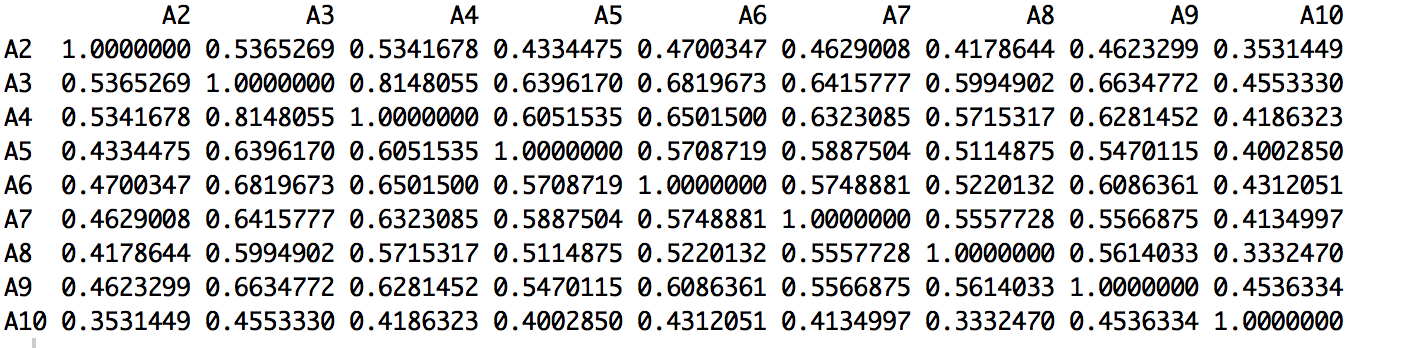
\includegraphics[width=0.7\linewidth]{correlation}
\caption{}
\label{fig:correlation}
\end{figure}
 \end{enumerate}
 \end{enumerate} 
  \item  Implement $k$-means so that you can cluster $\Delta_2^{clean}$ without using $C$.  Upon stopping, you will calculate the quality of the centroids and of the partition.  For each centroid $c_i$, form two counts:
  \begin{eqnarray*}
  b_i &\gets& \sum_{\delta \in c_i.B} [\delta.C = 2],\ \ \ \mbox{\rm benign}\\
  m_i &\gets& \sum_{\delta \in c_i.B} [\delta.C = 4], \ \ \ \mbox{\rm malignant}
  \end{eqnarray*}
  where $[x = y]$ returns 1 if True, 0 otherwise.  For example, $[2 = 3] + [0 = 0] + [34 = 34] = 2$
  
  The centroid $c_i$ is classified as benign if $b_i > m_i$ and malignant otherwise.  We can now calculate a simple error rate.    Assume $c_i$ is benign.  Then the error is:
 \begin{eqnarray*}
 error(c_i) &=& \frac{m_i}{m_i + b_i}
 \end{eqnarray*}
 We can find the total error rate easily:
 \begin{eqnarray*}
 Error(\{c_1, c_2, \ldots, c_k\}) &=& \sum_{i=1}^k error(c_i)
 \end{eqnarray*}

Report the total error rates for $k = 2,\ldots 5$ for 20 runs each, presenting the results that are easily understandable.  Plots are generally a good way to convey complex ideas quickly.  Discuss your results and include your initial problem statement. \\
Answer:\\
\begin{enumerate}
	\item When k = 2, I initialzed the centroid by choosen the two datapoint in the dataset which has the biggest distance in the all set. Then do the k-means. This part of code put in the txt file whin the java.zip file. For the reason that late k = 3, 4, 5 I implemented a method to initialzed the controids randomly from the data set.\\
	Use this method I got a very good result as $error\ = 0.032$\\
	However when I initialzed the centroids by randomly choose from the dataset, the $error$ is always around $0.1$.
	
	Which combined with the statement before. Gave us a conclusion. When we knew the cluster number before implemented the data. And we can make more customerlized centroid which might gave us a better result then we just randomly choose the centroid.
	\item when $k = 3$\\
	The answer for 20 runs is:\\
	0.60 0.61 0.57 0.37 0.23 0.17 0.17 0.17 0.16 0.17 0.17 0.17 0.17 0.17 0.17 0.17 0.17 0.17 0.17 0.17 
	\item when $k = 4$\\
	The answer for 20 runs is:\\
	0.49 0.27 0.19 0.15 0.16 0.15 0.15 0.15 0.15 0.15 0.15 0.15 0.15 0.15 0.15 0.15 0.15 0.15 0.15 0.15 
	\item when $k = 5$ \\
	The answer for 20 runs is:\\
	0.65 0.33 0.22 0.19 0.19 0.19 0.19 0.19 0.19 0.19 0.19 0.19 0.19 0.19 0.19 0.19 0.19 0.19 0.19 0.19
	\item Discussion:\\
	\begin{enumerate}
		\item When $k > 2$, the centroids are initialzed randomly from the dataset. And as I run more times the program. It seems like as then k getting bigger when result gets bigger too. which means the error gets bigger. But when we run many times. The result get down as the program get going.
		\item As I implement many times for different $k$, I found out that when $k$ is big as 4,5. It more likely gave us a big error number for example $0.86$ as so on. Which is unreasonable. So it probably would make the result unstable when $k$ is bigger than 3.
		\item As the $k$ gets bigger, as 6, 7, 8. The error getting bigger. And there is a funny thing comes out when $k$ keeping getting bigger as more than 10. Is would make some centroid assign to no datapoints. which means we may just pick useless datapoint for cluster.
		\item As the statement mentioned above. When $k$ getting bigger. It would be more likely that Centroid Collapse happes.
	\end{enumerate} 
\end{enumerate}

\end{enumerate}

\section*{What to Turn-in}
\begin{itemize}
\item The *pdf of the written answers to this document.
\item The code for $k$-means, \texttt{R}.
\item The AIs can schedule a time to verify your codes works.  If there is a subsequent time-stamp to the due date of the source code, the grade may be reduced.  
\end{itemize}
\bibliographystyle{unsrt} 
\bibliography{hw2}
\end{document}
